%!TEX program = xelatex
%Template created by: Maciej Byczko
\documentclass[a4paper,12pt]{extarticle}  %typ dokumentu

% \usepackage[utf8]{inputenc} %rodzaj czcionki w dokumencie
\usepackage{geometry} %poprawienie marginesów
\usepackage{polski} %polskie znaki
\usepackage{multirow} %tabela
\usepackage{graphicx} %tabela
\usepackage{float} %poprawienie pozycji
\usepackage{fancyhdr} % header i footer
\usepackage{karnaugh-map} % rysowanie siatek karnaugh
\usepackage{hyperref} %tworzenie odnośników, \url{<url>}, \href{<file path, link>}{<text with link>} \pageref{}
\usepackage{amsmath} % Matma
\usepackage{boldline}%edytowanie grubości krawędzi w tabelach \hlineB{} \clineB{}{}
\usepackage{array}%grubsze kolumny w tabeli
\usepackage{bigstrut}
\usepackage{caption}
\usepackage{listings} %pisanie kodu w ładny sposób, begin{listings}[language=<język>]...end{listings} tak samo jak nazwa paczki
\usepackage{subcaption}

%Ustawienie paczki hyperref
\hypersetup{
     colorlinks,
     citecolor=black,
     filecolor=black,
     linkcolor=black,
     urlcolor=black
}

\definecolor{backcolour}{rgb}{0.95,0.95,0.92}
\definecolor{AO}{rgb}{0,0.5,0}
\definecolor{ZeroBlue}{rgb}{0,0.28,0.73}
\definecolor{DarkRed}{rgb}{0.85,0.16,0.16}

\lstset{
breaklines=true,
language=vhdl,
numbers=left,
tabsize=2,
numberstyle=\tiny,
backgroundcolor=\color{backcolour},
breakatwhitespace=false,
showspaces=false,                
showstringspaces=false,
showtabs=false,
commentstyle=\color{gray},
keywordstyle=\color{ZeroBlue},
% keywordstyle={[2]\color{DarkRed}},
% keywordstyle={[3]\color{ZeroBlue}},
}
\graphicspath{{pictures/}}
\geometry{margin=0.7in}
\pagestyle{fancy}

\cfoot{Strona \thepage}
\rhead{Strona \thepage}
\lhead{\typdoc}
\newcolumntype{?}{!{\vrule width 1.5pt}}

\title{\tytul}
\author{\tworcy}
\date{\data}

%-----------------------PRZYDATNE LINKI----------------------------------
%link do tworzenia tabeli https://tablesgenerator.com
%symbole matematyczne: https://oeis.org/wiki/List_of_LaTeX_mathematical_symbols
%narzędzia matematyczne: https://en.wikibooks.org/wiki/LaTeX/Mathematics
%krótkie podpowiedzi http://www.mif.pg.gda.pl/homepages/sylas/students/wdi/doc/latex-sciaga.html
%symbole do schematów: http://texdoc.net/texmf-dist/doc/latex/circuitikz/circuitikzmanual.pdf
%----------------------------------------------------------------------

%-----------------------SEKCJA DANYCH----------------------------------
\def\tytul{Układy Sekwencyjne} %<<< tytuł ćwiczenia
\def\nrcw{2} %<<< numer ćwiczenia
\def\data{10 Października 2021} %<< data wykonania
\def\prowadzacy{dr inż. Jacek Mazurkiewicz} %<<<prowadzący
\def\nrgrupy{B} %<<<numer grupy
\def\tworcy{Maciej Byczko\\Bartosz Matysiak} %<<< autorzy
\def\zajinfo{PN 10:50 TP} %<<< informacje dotyczące zajęć
\def\typdoc{Sprawozdanie} %<<< typ dokumentu tj Sprawozdanie, zadania itp. {Matematyka dyskretna/Sprawozdanie z Miernictwa}
\begin{document}
\setlength{\headheight}{15pt}

\newcommand{\ov}[1]{\overline{#1} \ }

%-------------------------------------TABELA-DANYCH--------------------------------------------------
\begin{table}[H]
	\centering
	\resizebox{\textwidth}{!}{
		\begin{tabular}{|c|c|c|}\hline
			\begin{tabular}[c]{@{}c@{}}                     \tworcy     \end{tabular} &
			\begin{tabular}[c]{@{}c@{}}Prowadzący:\\        \prowadzacy \end{tabular} &
			\begin{tabular}[c]{@{}c@{}}Numer ćwiczenia\\    \nrcw       \end{tabular}          \\ \hline
			\begin{tabular}[c]{@{}c@{}}                     \zajinfo    \end{tabular} &
			\begin{tabular}[c]{@{}c@{}}Temat ćwiczenia:\\   \tytul      \end{tabular} & Ocena: \\ \hline
			\begin{tabular}[c]{@{}c@{}}Grupa:\\          \nrgrupy    \end{tabular}    &
			\begin{tabular}[c]{@{}c@{}}Data wykonania:\\    \data       \end{tabular} &        \\ \hline
		\end{tabular}}
\end{table}
%----------------------------------------------------------------------------------------------------
\tableofcontents
\cleardoublepage
\section{Zadanie 1}
\subsection{Polecenie}
Zaprojektować licznik synchroniczny liczący w tył na bazie kodu Aikena w zakresie 0-6 (mod 7).
% Licznik synchroniczny, mod 7, negatywny, kod Aikena
\subsection{Rozwiązanie}
\subsubsection{Schemat stanów}
\begin{figure}[H]
	\centering
	\resizebox*{0.65\textwidth}{!}{
		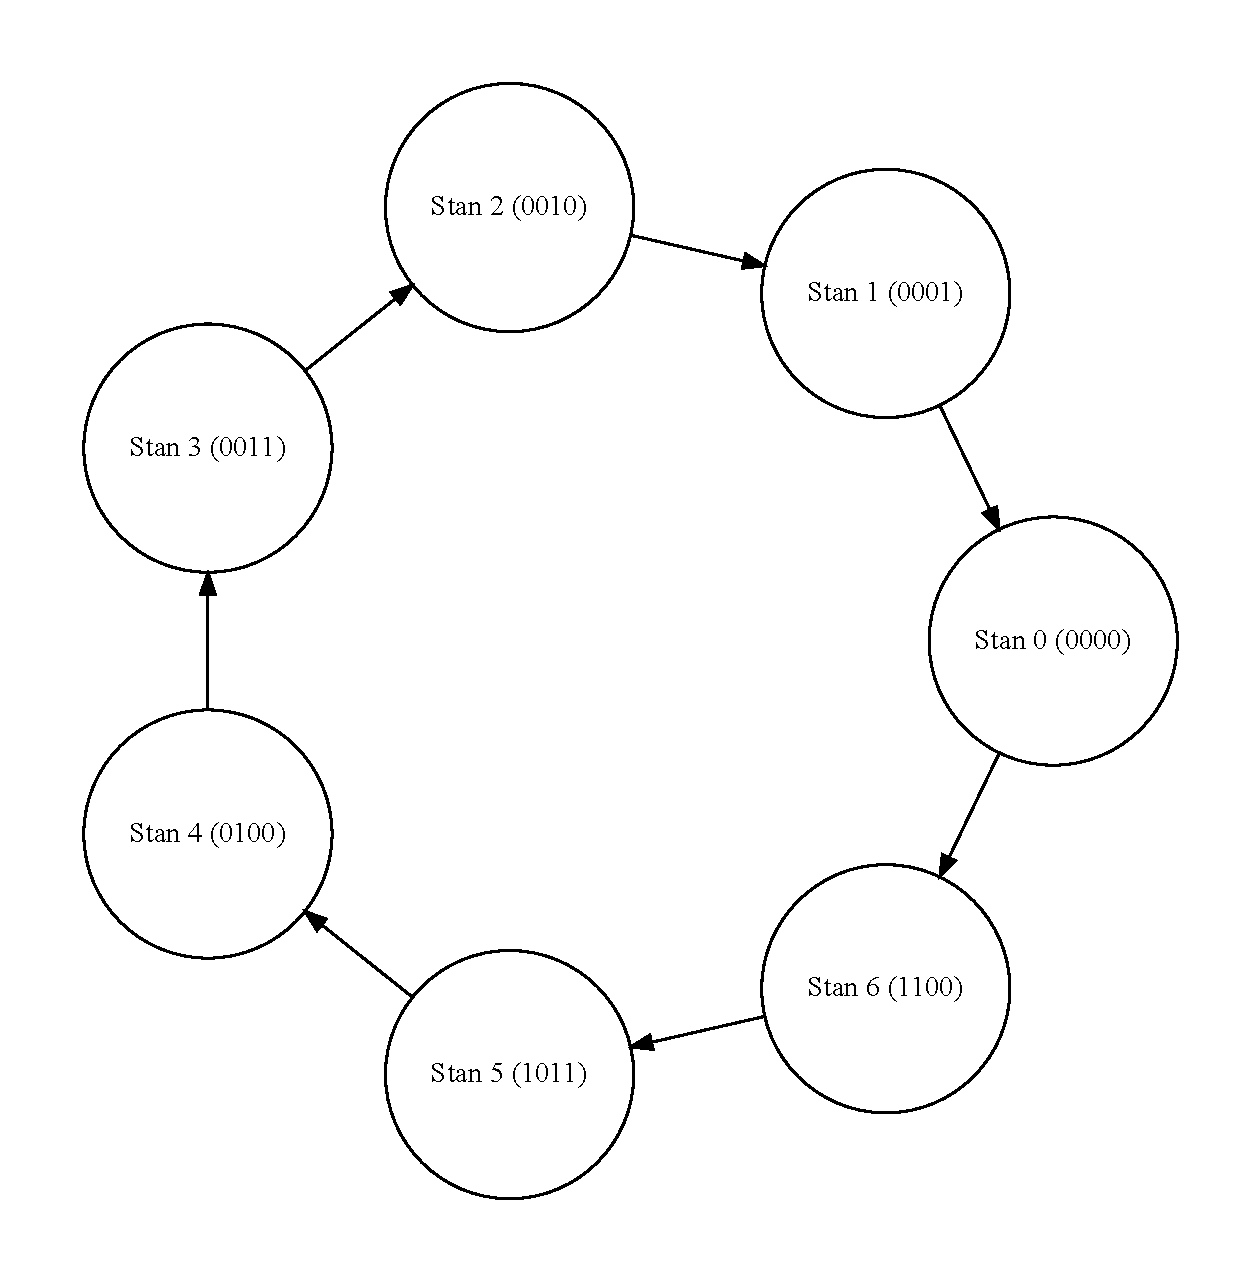
\includegraphics{zadanie1/stany.pdf}
	}
\end{figure}
\subsubsection{Tabela prawdy}
% Table generated by Excel2LaTeX from sheet 'Sheet1'
\begin{table}[H]
	\centering
	% \caption{Add caption}
	% \centering
	\resizebox*{\textwidth}{!}{
		\begin{tabular}{|c?c|c|c|c?c|c|c|c?c|c|c|c|c|c|c|c|}
			\hline
			\multirow{2}[3]{*}{n} & \multicolumn{4}{c?}{Q(t)} & \multicolumn{4}{c?}{Q(t+1)} & \multicolumn{8}{c|}{JK} \bigstrut                                                                                                                    \\
			\clineB{2-17}{2.5}    & $Q_3$                     & $Q_2$                       & $Q_1$                             & $Q_0$ & $Q_3$ & $Q_2$ & $Q_1$ & $Q_0$ & $J_3$ & $K_3$ & $J_2$ & $K_2$ & $J_1 $ & $K_1$ & $J_0$ & $K_0$ \bigstrut \\
			\hlineB{2.5}
			0                     & 0                         & 0                           & 0                                 & 0     & 1     & 1     & 0     & 0     & 1     & -     & 1     & -     & 0      & -     & 0     & - \bigstrut     \\
			\hline
			1                     & 0                         & 0                           & 0                                 & 1     & 0     & 0     & 0     & 0     & 0     & -     & 0     & -     & 0      & -     & -     & 1 \bigstrut     \\
			\hline
			2                     & 0                         & 0                           & 1                                 & 0     & 0     & 0     & 0     & 1     & 0     & -     & 0     & -     & -      & 1     & 1     & - \bigstrut     \\
			\hline
			3                     & 0                         & 0                           & 1                                 & 1     & 0     & 0     & 1     & 0     & 0     & -     & 0     & -     & -      & 0     & -     & 1 \bigstrut     \\
			\hline
			4                     & 0                         & 1                           & 0                                 & 0     & 0     & 0     & 1     & 1     & 0     & -     & -     & 1     & 1      & -     & 1     & - \bigstrut     \\
			\hline
			5                     & 1                         & 0                           & 1                                 & 1     & 0     & 1     & 0     & 0     & -     & 1     & 1     & -     & -      & 1     & -     & 1 \bigstrut     \\
			\hline
			6                     & 1                         & 1                           & 0                                 & 0     & 1     & 0     & 1     & 1     & -     & 0     & -     & 1     & 1      & -     & 1     & - \bigstrut     \\
			\hline
		\end{tabular}%
	}
	\label{tab:states}%
\end{table}%
\subsubsection{Siatki Karnaugh}
\begin{figure}[H]
\centering
\begin{minipage}[c]{0.49\linewidth}
\begin{karnaugh-map}[4][4][1][$Q_1Q_0$][$Q_3Q_2$]
\minterms{0} % na tych koordynatach umieść jedynki (1)
\maxterms{1,2,3,4}
\autoterms[-] % umieść ten symbol w miejscach niezdefiniowanych
\implicantedge{0}{0}{8}{8}
\end{karnaugh-map}
\centering
\vspace{-1cm}
\hspace{1cm}
\caption*{$J_3 = \ov{Q_2}\ov{Q_1}\ov{Q_0}$}
\end{minipage}
\centering
\begin{minipage}[c]{0.49\linewidth}
\begin{karnaugh-map}[4][4][1][$Q_1Q_0$][$Q_3Q_2$]
\minterms{0,11} % na tych koordynatach umieść jedynki (1)
\maxterms{1,2,3}
\autoterms[-] % umieść ten symbol w miejscach niezdefiniowanych
\implicant{0}{8}
\implicant{12}{10}
\end{karnaugh-map}
\centering
\vspace{-1cm}
\hspace{1cm}
\caption*{$J_2 = \ov{Q_1}\ov{Q_0} + Q_3$}
\end{minipage}
\end{figure}
\vspace{-1cm}
\begin{figure}[H]
\centering
\begin{minipage}[c]{0.49\linewidth}
\begin{karnaugh-map}[4][4][1][$Q_1Q_0$][$Q_3Q_2$]
\minterms{4,12} % na tych koordynatach umieść jedynki (1)
\maxterms{0,1}
\autoterms[-] % umieść ten symbol w miejscach niezdefiniowanych
\implicant{4}{14}
\end{karnaugh-map}
\centering
\vspace{-1cm}
\hspace{1cm}
\caption*{$J_1 = Q_2$}
\end{minipage}
\centering
\begin{minipage}[c]{0.49\linewidth}
\begin{karnaugh-map}[4][4][1][$Q_1Q_0$][$Q_3Q_2$]
\minterms{2,4,12} % na tych koordynatach umieść jedynki (1)
\maxterms{0}
\autoterms[-] % umieść ten symbol w miejscach niezdefiniowanych
\implicant{4}{14}
\implicant{3}{10}
\end{karnaugh-map}
\centering
\vspace{-1cm}
\hspace{1cm}
\caption*{$J_0 = Q_1 + Q_2$}
\end{minipage}
\vspace{-0.1cm}
\end{figure}
\vspace{-1cm}
%? Siatki dla K
\begin{figure}[H]
\centering
\begin{minipage}[c]{0.49\linewidth}
\begin{karnaugh-map}[4][4][1][$Q_1Q_0$][$Q_3Q_2$]
\minterms{11} % na tych koordynatach umieść jedynki (1)
\maxterms{12}
\autoterms[-] % umieść ten symbol w miejscach niezdefiniowanych
% \implicantedge{0}{0}{8}{8}
\implicant{3}{10}
%\implicant{1}{11}
%\implicantedge{0}{2}{8}{10}
\end{karnaugh-map}
\centering
\vspace{-1cm}
\hspace{1cm}
\caption*{$K_3 = Q_1$} %* Wybierz jedno
\end{minipage}
\centering
\begin{minipage}[c]{0.49\linewidth}
\begin{karnaugh-map}[4][4][1][$Q_1Q_0$][$Q_3Q_2$]
\minterms{4,12} % na tych koordynatach umieść jedynki (1)
\maxterms{}
\autoterms[-] % umieść ten symbol w miejscach niezdefiniowanych
\implicant{0}{10}
% \implicant{12}{10}
\end{karnaugh-map}
\centering
\vspace{-1cm}
\hspace{1cm}
\caption*{$K_2 = 1$}
\end{minipage}
\end{figure}
\vspace{-1cm}
\begin{figure}[H]
\centering
\begin{minipage}[c]{0.49\linewidth}
\begin{karnaugh-map}[4][4][1][$Q_1Q_0$][$Q_3Q_2$]
\minterms{2,11} % na tych koordynatach umieść jedynki (1)
\maxterms{3}
\autoterms[-] % umieść ten symbol w miejscach niezdefiniowanych
% \implicant{4}{14}
\implicantedge{0}{8}{2}{10}
\implicant{12}{10}
\end{karnaugh-map}
\centering
\vspace{-1cm}
\hspace{1cm}
\caption*{$K_1 = \ov{Q_0} + Q_3$}
\end{minipage}
\centering
\begin{minipage}[c]{0.49\linewidth}
\begin{karnaugh-map}[4][4][1][$Q_1Q_0$][$Q_3Q_2$]
\minterms{1,3,11} % na tych koordynatach umieść jedynki (1)
% \maxterms{}
\autoterms[-] % umieść ten symbol w miejscach niezdefiniowanych
% \implicant{4}{14}
% \implicant{3}{10}
\implicant{0}{10}
\end{karnaugh-map}
\centering
\vspace{-1cm}
\hspace{1cm}
\caption*{$K_0 = 1$}
\end{minipage}
\end{figure}
\subsubsection{Schemat układu}
\begin{figure}[H]
	\centering
	\resizebox*{\textwidth}{!}{
		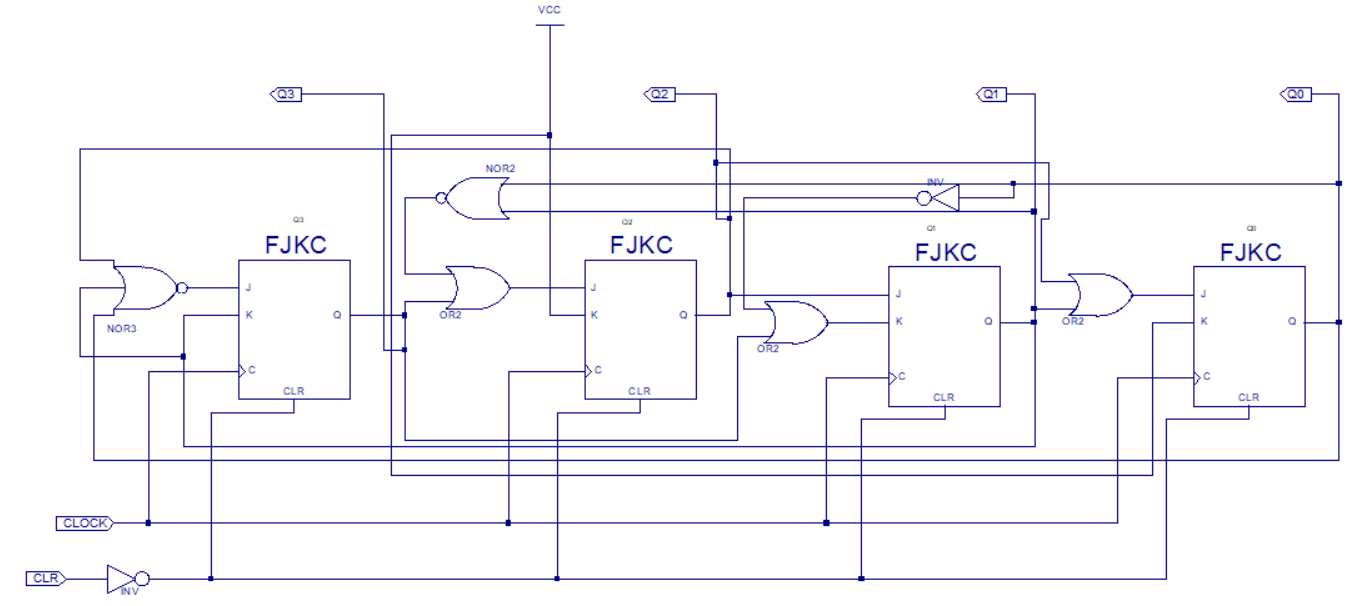
\includegraphics{zadanie1/zad1_schematic.png}
	}
\end{figure}
\subsubsection{Kod VHDL}
\lstinputlisting{zadanie1/zad1.vhd}
\subsubsection{Symulacja}
\begin{figure}[H]
	\centering
	\resizebox*{\textwidth}{!}{
		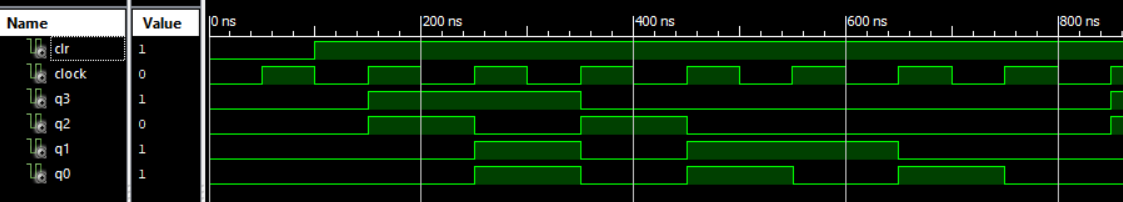
\includegraphics{zadanie1/zad1_simulation_v2.png}
	}
\end{figure}
UWAGA: Powyższy przebieg przedstawia działanie układu licznika rozpoczęte stanem ''0000''.
\subsubsection{Plik ucf}
\lstinputlisting{zadanie1/zad1.ucf}
\section{Zadanie 2}
\subsection{Polecenie}
Detektor sekwencji 11011, automat Mealy-ego, jedno wejście, jedno wyjście, brak resetu, sekwencja prawidłowa 5-bitowa.
\subsection{Rozwiązanie}
\subsubsection{Opis symboliki}
\textbf{Alfabet wejściowy}
\begin{itemize}
    \item $z_0 = 0$
    \item $z_1 = 1$
\end{itemize}
\textbf{Stany wewnętrzne}
\begin{itemize}
    \item $q_0$ - stan początkowy | wprowadzono niepoprawny ciąg bitów
    \item $q_1$ - wprowadzono pierwszą cyfrę prawidłowego ciągu
    \item $q_2$ - wprowadzono drugą cyfrę prawidłowego ciągu
    \item $q_3$ - wprowadzono trzecią cyfrę prawidłowego ciągu
    \item $q_4$ - wprowadzono czwartą cyfrę prawidłowego ciągu
    \item $q_5$ - wprowadzono poprawną sekwencję
\end{itemize}
\textbf{Alfabet wyjścia}
\begin{itemize}
    \item $y_0$ - Wprowadzony ciąg nadal jest niepoprawny
    \item $y_1$ - Wprowadzono poprawną sekwencję
\end{itemize}
\subsubsection{Schemat grafowy}
\begin{figure}[H]
	\centering
	\resizebox*{\textwidth}{!}{
		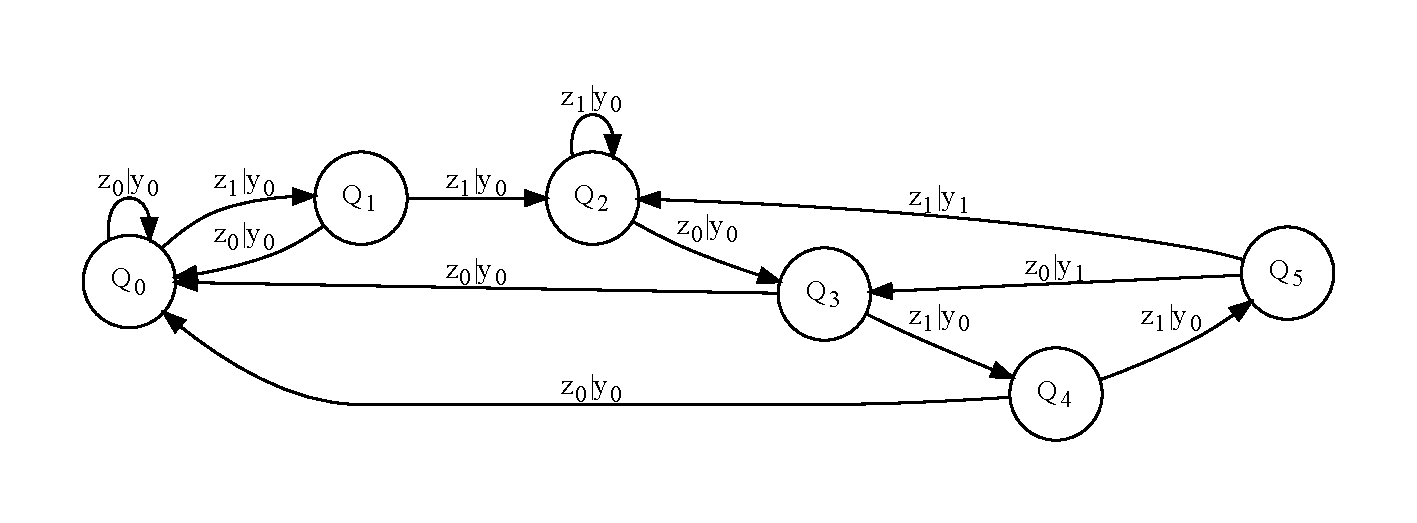
\includegraphics{zadanie2/mealy.pdf}
	}
\end{figure}
\subsubsection{Tabela prawdy}
% Table generated by Excel2LaTeX from sheet 'Sheet1'
% Table generated by Excel2LaTeX from sheet 'Sheet1'
\begin{table}[H]
    \centering
    % \caption{Add caption}
    \resizebox*{\textwidth}{!}{
      \begin{tabular}{|c?c|c|c?c?c|c|c?c?c|c|c|}
      \hline
      \multirow{2}[4]{*}{S} & \multicolumn{3}{c?}{Q(t)} & \multirow{2}[4]{*}{Z} & \multicolumn{3}{c?}{Q(t+1)} & \multirow{2}[4]{*}{Y} & \multicolumn{3}{c|}{T(t)} \bigstrut\\
  \clineB{2-4}{2.5}\clineB{6-8}{2.5}\clineB{10-12}{2.5}      & $Q_2$ & $Q_1$ & $Q_0$ &   & $Q_2$ & $Q_1$ & $Q_0$ &   & $T_2$ & $T_1$ & $T_0$ \bigstrut\\
      \hlineB{2.5}
      $Q_0$ & 0 & 0 & 0 & 0 & 0 & 0 & 0 & 0 & 0 & 0 & 0 \bigstrut\\
      \hline
      $Q_0$ & 0 & 0 & 0 & 1 & 0 & 0 & 1 & 0 & 0 & 0 & 1 \bigstrut\\
      \hline
      $Q_1$ & 0 & 0 & 1 & 0 & 0 & 0 & 0 & 0 & 0 & 0 & 1 \bigstrut\\
      \hline
      $Q_1$ & 0 & 0 & 1 & 1 & 0 & 1 & 0 & 0 & 0 & 1 & 1 \bigstrut\\
      \hline
      $Q_2$ & 0 & 1 & 0 & 0 & 0 & 1 & 1 & 0 & 0 & 0 & 1 \bigstrut\\
      \hline
      $Q_2$ & 0 & 1 & 0 & 1 & 0 & 1 & 0 & 0 & 0 & 0 & 0 \bigstrut\\
      \hline
      $Q_3$ & 0 & 1 & 1 & 0 & 0 & 0 & 0 & 0 & 0 & 1 & 1 \bigstrut\\
      \hline
      $Q_3$ & 0 & 1 & 1 & 1 & 1 & 0 & 0 & 0 & 1 & 1 & 1 \bigstrut\\
      \hline
      $Q_4$ & 1 & 0 & 0 & 0 & 0 & 0 & 0 & 0 & 1 & 0 & 0 \bigstrut\\
      \hline
      $Q_4$ & 1 & 0 & 0 & 1 & 1 & 0 & 1 & 0 & 0 & 0 & 1 \bigstrut\\
      \hline
      $Q_5$ & 1 & 0 & 1 & 0 & 0 & 1 & 1 & 1 & 1 & 1 & 0 \bigstrut\\
      \hline
      $Q_5$ & 1 & 0 & 1 & 1 & 0 & 1 & 0 & 1 & 1 & 1 & 1 \bigstrut\\
      \hline
      - & 1 & 1 & 0 & 0 & - & - & - & - & - & - & - \bigstrut\\
      \hline
      - & 1 & 1 & 0 & 1 & - & - & - & - & - & - & - \bigstrut\\
      \hline
      - & 1 & 1 & 1 & 0 & - & - & - & - & - & - & - \bigstrut\\
      \hline
      - & 1 & 1 & 1 & 1 & - & - & - & - & - & - & - \bigstrut\\
      \hline
      \end{tabular}%
    }
    \label{tab:mealy}%
  \end{table}%
  
\subsubsection{Siatka Karnaugh}
\begin{figure}[H]
    \centering
    \begin{minipage}[c]{0.49\linewidth}
    \begin{karnaugh-map}[4][4][1][$Q_0Z$][$Q_2Q_1$]
    \minterms{7,8,10,11}
    \maxterms{0,1,2,3,4,5,6,9}
    \autoterms[-] % umieść ten symbol w miejscach niezdefiniowanych
    \implicant{7}{15}
    \implicantedge{12}{8}{14}{10}
    \implicant{15}{10}
    % \minterms{0} % na tych koordynatach umieść jedynki (1)
    % \maxterms{1,2,3,4}
    % \implicantedge{0}{0}{8}{8}
    \end{karnaugh-map}
    \centering
    \vspace{-1cm}
    \hspace{1cm}
    \caption*{$T_2 = Q_1Q_0Z + Q_2\ov{Z} + Q_2Q_0$}
    \end{minipage}
    \centering
    \begin{minipage}[c]{0.49\linewidth}
    \begin{karnaugh-map}[4][4][1][$Q_0Z$][$Q_2Q_1$]
    \minterms{3,6,7,10,11}
    \maxterms{0,1,2,4,5,8,9}
    \autoterms[-] % umieść ten symbol w miejscach niezdefiniowanych
    \implicant{3}{11}
    \implicant{7}{14}
    \implicant{15}{10}
    % \minterms{0,11} % na tych koordynatach umieść jedynki (1)
    % \maxterms{1,2,3}
    % \implicant{0}{8}
    % \implicant{12}{10}
    \end{karnaugh-map}
    \centering
    \vspace{-1cm}
    \hspace{1cm}
    \caption*{$T_1 = Q_0Z + Q_1Q_0 + Q_2Q_0$}
    \end{minipage}
    \end{figure}
    \vspace{-1cm}
    \begin{figure}[H]
    \centering
    \begin{minipage}[c]{0.49\linewidth}
    \begin{karnaugh-map}[4][4][1][$Q_0Z$][$Q_2Q_1$]
    \minterms{1,2,3,4,6,7,9,11}
    \maxterms{0,5,8,10}
    \implicant{3}{6}
    \implicantedge{4}{12}{6}{14}
    \implicantedge{1}{3}{9}{11}
    % \minterms{4,12} % na tych koordynatach umieść jedynki (1)
    % \maxterms{0,1}
    \autoterms[-] % umieść ten symbol w miejscach niezdefiniowanych
    % \implicant{4}{14}
    \end{karnaugh-map}
    \centering
    \vspace{-1cm}
    \hspace{1cm}
    \caption*{$T_0 = \ov{Q_2}Q_0 + Q_1\ov{Z} + \ov{Q_1}Z$}
    \end{minipage}
    \begin{minipage}[c]{0.49\linewidth}
        \begin{karnaugh-map}[4][4][1][$Q_0Z$][$Q_2Q_1$]
        \minterms{10,11}
        \maxterms{0,1,2,3,4,5,6,7,8,9}
        \implicant{15}{10}
        % \minterms{4,12} % na tych koordynatach umieść jedynki (1)
        % \maxterms{0,1}
        \autoterms[-] % umieść ten symbol w miejscach niezdefiniowanych
        % \implicant{4}{14}
        \end{karnaugh-map}
        \centering
        \vspace{-1cm}
        \hspace{1cm}
        \caption*{$Y = Q_2Q_0 $}
        \end{minipage}
    % \centering
    % \begin{minipage}[c]{0.49\linewidth}
    % \begin{karnaugh-map}[4][4][1][$Q_1Q_0$][$Q_3Q_2$]
    % \minterms{2,4,12} % na tych koordynatach umieść jedynki (1)
    % \maxterms{0}
    % \autoterms[-] % umieść ten symbol w miejscach niezdefiniowanych
    % \implicant{4}{14}
    % \implicant{3}{10}
    % \end{karnaugh-map}
    % \centering
    % \vspace{-1cm}
    % \hspace{1cm}
    % \caption*{$J_0 = Q_1 + Q_2$}
    % \end{minipage}
    % \vspace{-0.1cm}
    \end{figure}

    \subsubsection{Schemat układu}
    \begin{figure}[H]
        \centering
        \resizebox*{\textwidth}{!}{
            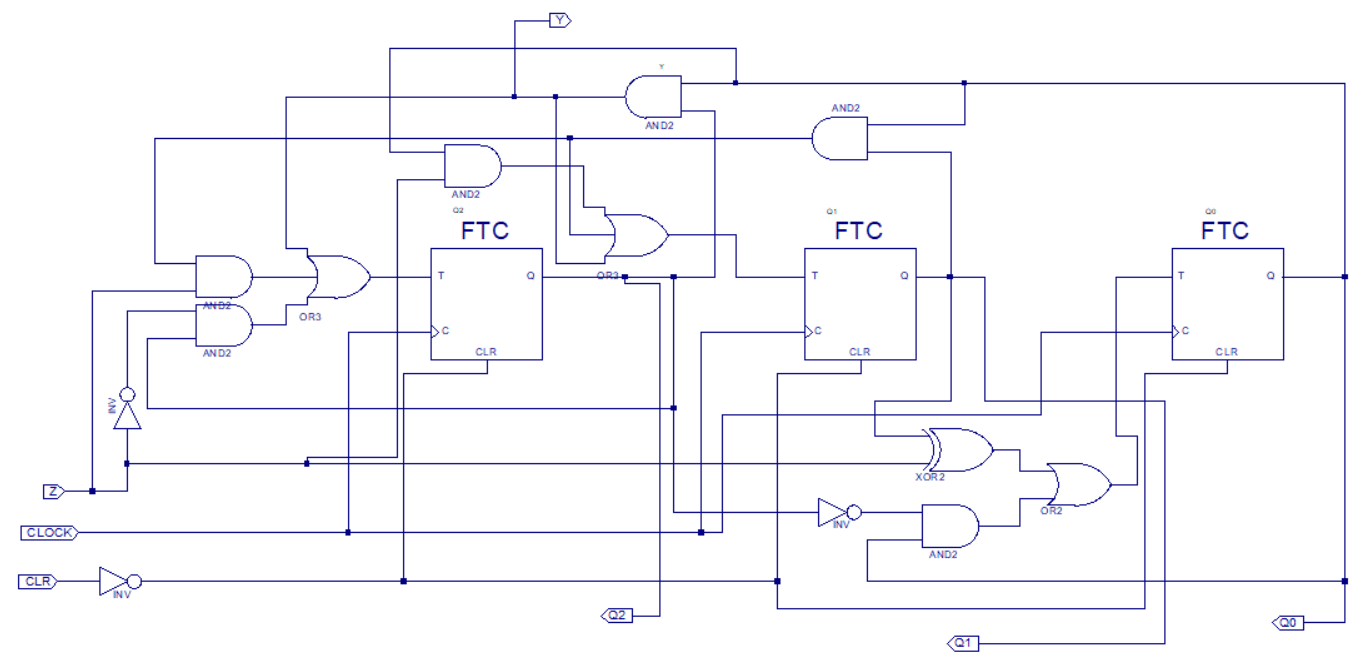
\includegraphics{zadanie2/zad2_schematic.png}
        }
    \end{figure}
    \subsubsection{Kod VHDL}
    \lstinputlisting{zadanie2/MealyDetectorTestBenchqucker.vhd}
    \subsubsection{Symulacja}
    \begin{figure}[H]
        \centering
        \resizebox*{\textwidth}{!}{
            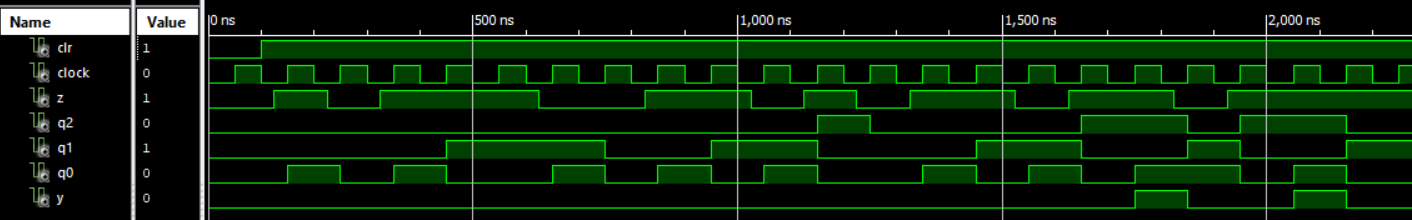
\includegraphics{zadanie2/zad2_simulation_v2.png}
        }
    \end{figure}
    UWAGA: Powyższy przebieg obrazuje przejście po każdej krawędzi rozpatrywanego grafu automatu Mealy'ego. Przejście do nowego stanu automatu realizuje się w momencie wystąpienia zbocza wznoszącego na wejściu CLOCK. Z przebiegu można odczytać m.in. to, że sekwencja prawidłowa ''11011'' została w przebiegu wykryta dwukrotnie, a także, że w chwili $t = 475 ns$ układ znajdował się w stanie $q_2$, i nie akceptował bieżącej sekwencji.
    \subsubsection{Plik ucf}
    \lstinputlisting{zadanie2/zad2.ucf}
\section{Wnioski}

Przy wykonywaniu zadań niezbędna okazała się wiedza na temat typów przerzutników i ich działania. Oprócz tego, ćwiczenia wymagały także zapoznania się z opracowaniem dotyczącym zestawu ZL-9572, a konkretniej - generatorów sygnałów prostokątnych \textbf{Clk\_XT} i \textbf{Clk\_LF} oraz modułu czterocyfrowego wyświetlacza siedmiosegmentowego. \\
Pierwsze zadanie dotyczyło stworzenia licznika negatywnego modulo 7 zliczającego w kodzie Aikena. Wykorzystaliśmy w jego rozwiązaniu przerzutniki JK, a konkretnie komponenty FJKC z biblioteki programu Xilinx, przyjmując przy okazji założenie, że praca licznika rozpoczyna się od jego resetu (sprowadzenia do stanu ''0000''), który należało zrealizować, czy to poprzez uaktywnienie sygnału CLR na etapie symulacji, czy naciśnięcie odpowiednio przypisanego przycisku w implementacji sprzętowej. Alternatywnie możliwe byłoby także wykorzystanie komponentów FJKP bądź FJKCP, gdyby zachodziła konieczność stworzenia układu rozpoczynającego pracę w innym stanie początkowym. \\
Podobne założenie dotyczące pochodzenia stanu początkowego przyjęliśmy także w zadaniu 2. Należało w nim stworzyć układ detektora sekwencji ''11011'' oparty na automacie Mealy'ego. Przyjęliśmy, że układ prawidłowo reaguje na dowolnie długą sekwencję, o ile kończy się ona wcześniej wspomnianą, 5-bitową; możliwe jest w szczególności kilkukrotne wykrycie poprawnej sekwencji w trakcie pracy układu. \\
W rozszerzonej wersji, zadanie 2 należało rozszerzyć o obsługę wejścia przy pomocy modułu Rotary Encoder, a także prezentację aktualnego stanu układu przy pomocy wyświetlacza siedmiosegmentowego. Niestety, nie udało się zrealizować tej wersji zadania w całości: powiodło się zaimportowanie plików z gotowymi modułami do projektu. Wykorzystujący je schemat okazał się jednak niesyntezowalny. Podejrzewamy, że może mieć to związek z niepoprawnym użyciem przez nas magistrali i błędnym przyporządkowaniem pojedynczych ścieżek w niej zawartych. 

\end{document}